% Energy based spectrum sensing
\section{Energy based Spectrum Detector for Multiple Primary Users}
\subsection{System Model}
We consider a cognitive radio system where the licensed frequency spectrum could be occupied by exactly one of two distinct signals $\{s_1, s_2\}$ or it could be vacant. Let $H_0$ denote the hypothesis under which the channel is free, ${H}_1$ denote the hypothesis under which the channel is occupied by $s_1$ and ${H}_2$ denote the hypothesis under which the channel is occupied by $s_2$. We are interested to test $H_0$ against $\bar{{H}_0}$, where $\bar{H}_0$ denotes the hypothesis under which the channel is not free, using MENP framework.

A block diagram of the system is illustrated in Figure \ref{pic: block diagram}.

\begin{figure}[!hbp]
\centering
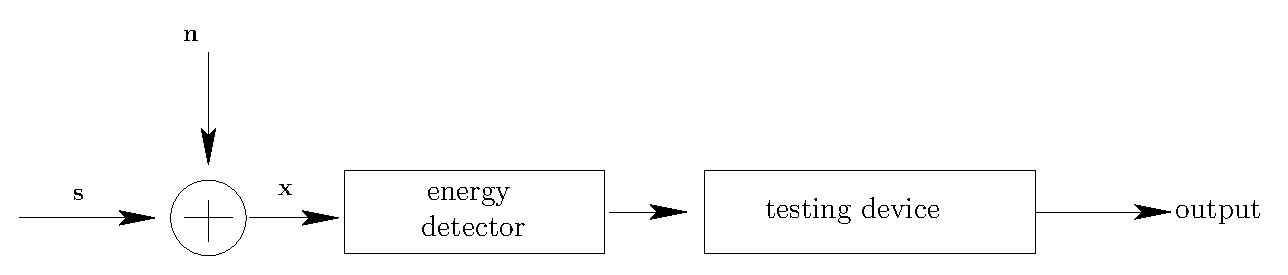
\includegraphics[width = \textwidth]{4/fig4.eps}
\caption{Block Diagram for Spectrum Sensing}
\label{pic: block diagram}
\end{figure}

The detector consists a measuring device followed by a testing device. 
The measuring device observes the noisy version of the signals that could present in the channel and outputs the sum energy of the sampled signals.
With this energy, the testing device employs MENP framework to decide about the state of the channel.
The input to the measuring device is 
\begin{equation}
  x[n] = 
  \begin{cases}
	\omega[n]\;\;\;\;\;\;&\text{when ${H}_0$ is true}\\
	s_1[n]+\omega[n]\;\;\;\;\;\;&\text{when ${H}_1$ is true}\\
	s_2[n]+\omega[n]\;\;\;\;\;\;&\text{when ${H}_2$ is true}
  \end{cases}
\end{equation}
where $n = \{0, \ldots, N-1\}$ are observation instance. 
We assume  $s_i[n]\;\;(i=1, 2)$ and $\omega[n]$ are zero-mean independent and identically distributed (iid) circularly symmetric complex Gaussian (CSCG) random variables with variances $2\sigma_{s_i}^2\;\;(i=1, 2)$ and $2\sigma_{\omega}^2$, i.e., $s_m[n] \sim \mathcal{CN}(0, 2\sigma_{s_i}^2)\;\;(i=1, 2)$ and $\omega[n] \sim \mathcal{CN}(0, 2\sigma_{\omega}^2)$.
Each noisy sample $x[n] = s_i[n] + \omega[n]$ is governed by a probability law under each hypothesis. In our model
since the noise and signal are independent, $s_i[n]+\omega[n] \sim \mathcal{CN}(0, 2(\sigma_{s_i}^2 + \sigma_\omega^2))$.  Define $\sigma_0^2 = \sigma_\omega^2$ and $\sigma_i^2 = \sigma_{s_i}^2 + \sigma_\omega^2$, we can see
\begin{equation}
  \label{1129a1}
  \begin{split}
  \omega[n] &\sim \mathcal{CN}(0, 2\sigma_0^2)\\
  \omega[n] + s_1[n]&\sim \mathcal{CN}(0, 2\sigma_1^2)\\
  \omega[n] + s_2[n]&\sim \mathcal{CN}(0, 2\sigma_2^2) \,,
  \end{split}
\end{equation}
thus the distribution of $x[n]$ under each hypothesis is given by
\begin{equation}
   \begin{split}
  H_0:\;\;\;\;\begin{pmatrix} x_R[n] \\ x_I[n] \end{pmatrix} \sim \mathcal{N}\Big( \begin{bmatrix} 0 \\ 0 \end{bmatrix}, \begin{bmatrix} \sigma_0^2 & 0\\ 0 & \sigma_0^2 \end{bmatrix} \Big)\\
  H_1:\;\;\;\;\begin{pmatrix} x_R[n] \\ x_I[n] \end{pmatrix} \sim \mathcal{N}\Big( \begin{bmatrix} 0 \\ 0 \end{bmatrix}, \begin{bmatrix} \sigma_1^2 & 0\\ 0 & \sigma_1^2 \end{bmatrix} \Big)\\
  H_2:\;\;\;\;\begin{pmatrix} x_R[n] \\ x_I[n] \end{pmatrix} \sim \mathcal{N}\Big( \begin{bmatrix} 0 \\ 0 \end{bmatrix}, \begin{bmatrix} \sigma_2^2 & 0\\ 0 & \sigma_2^2 \end{bmatrix} \Big)
\end{split}
  \label{equ:xdistribution}
\end{equation}
where $x_R[n]$ and $x_I[n]$ are real and imaginary component of signal $x[n]$.
In our case, the measuring device is an energy detector, the output is given by
\begin{equation} 
  Y = \sum_{n=0}^{N-1}|x[n]|^2 = \sum_{n=0}^{N-1}(x_R[n]^2+x_I[n]^2)\,.
  \label{equ: testing device}
\end{equation}
By observing $y$, a realization of $Y$, the testing device determines the status of the channel. 
Since $x_R[n], x_I[n]$ are uncorrelated Gaussian random variable with zero mean and variance $\sigma_i^2$, $\frac{y}{\sigma_i^2} = \sum_{n=0}^{N-1}((\frac{x_R[n]}{\sigma_i})^2 + (\frac{x_I[n]^2}{\sigma_i})^2)$ is governed by a Chi-Square distribution with $2N$ freedom degree under hypothesis $H_i$.
Hence the distribution of $Y$ can be expressed as:
\begin{equation} 
  \label{equ: abstract}
  \begin{split}
	H_0:\;\;\;\;&\frac{Y}{\sigma_0^2}\sim \mathcal{X}(2N)\\
	H_1:\;\;\;\;&\frac{Y}{\sigma_1^2}\sim \mathcal{X}(2N)\\
	H_2:\;\;\;\;&\frac{Y}{\sigma_2^2}\sim \mathcal{X}(2N)\,,
  \end{split}
\end{equation}
where $\mathcal{X}(2N)$ is the Chi-square distribution with $2N$ degree freedom. 

Let $P_d$ denote the probability of detection, i.e. the probability that the channel is correctly declared vacant ($H_0$ is correctly declared true) and $P_{f_i}$ denote the probability of false alarm with respect to $s_i$ ($i = 1, 2$), i.e. the probability that the channel is declared vacant when signal $s_i$ ($i = 1, 2$) is transmitting. Let $c_i$ ($i = 1, 2$) denotes the specific positive constraints on the probability of false alarm. The performance of the system can be depicted by $P_d$ and $c_i$ ($i = 1, 2$), and we use MENP framework to solve following optimization problem:
\begin{equation}
  \begin{split}
	\max\;\;\;\;&P_d\\
	\text{s.t.}\;\;\;\;&P_{f_1}\leq c_1\\
	&P_{f_2} \leq c_2\,.
  \end{split}
  \label{1129a3}
\end{equation}
Our goal is to plot M-ROC surface and to find the decision rule for a given $c_1, c_2$ value.

\subsection{Numerical Results}
From the definition of $\sigma_0^2, \sigma_1^2$ and $\sigma_2^2$, we know $\sigma_0^2 < \sigma_1^2, \sigma_2^2$. Hence  problem given in \eqref{1129a3} under hypotheses \eqref{equ: abstract} has the same form as that of Chi-Square Example given in last chapter. 
If $y$ is an observation of $Y$, 
from the conclusion in last chapter the optimal  decision rule for a given $c_1, c_2$ is 
\begin{equation}
  y \substack{H_0 \\ < \\ > \\ \bar{H}_0} V_\tau
  \label{equ:1129a4}
\end{equation}
where $V_\tau = \min\{F_1^{-1}(c_1),  F_2^{-1}(c_2)\}$ and function $F_1,  F_2$ are the CDFs of $Y$ under hypothesis $H_1, H_2$ respectively. The expression of $P_d$ is 
\begin{equation}
  P_d = F_0(V_\tau)\,.
  \label{equ:1129a5}
\end{equation}

Similar to energy detection in binary hypothesis testing, energy detection for multiple hypothesis testing differentiates between $H_0$ and $\bar{H}_0$ by comparing the test statistic (in form of energy) with a threshold $V_\tau$. The value of the threshold can be determined by the probability of false alarm constraints.  

We use Matlab to compute the M-ROC for this energy detector. The value of $c_1, c_2$ range from 0 to 0.1 with step 0.001. By using \eqref{equ:1129a4} and \eqref{equ:1129a5}, the value of $P_d$ can be acquired. The M-ROC is illustrate in Figure. \ref{pic:1201a1}.  

\begin{figure}[!t]
\centering
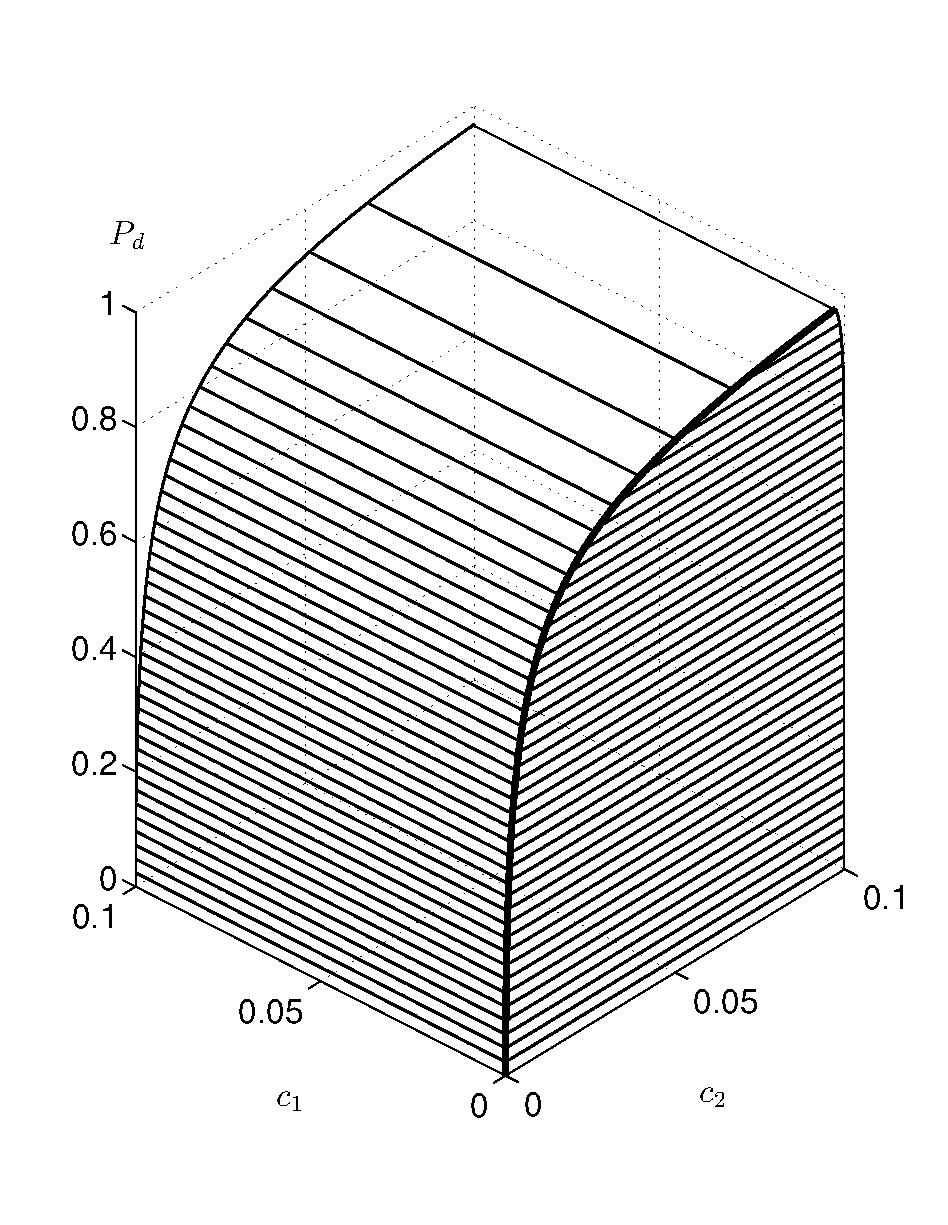
\includegraphics[width=12cm, height=16cm]{4/energy.eps}
\caption{M-ROC surface for $\sigma_\omega^2 = 0.1$, $\sigma_{s_1}^2=0.05$, $\sigma_{s_3}^2=0.15$ and $N = 20$.}
\label{pic:1201a1}
\end{figure}

